% Uncomment this to make slides with overlays:
%\documentclass[slides]{beamer}

% Uncomment these (but comment the above \documentclass line) to make handouts:
\documentclass[handout]{beamer}

% Uncomment these to have more than one slide per page
%\usepackage{pgfpages}
%\pgfpagesuselayout{2 on 1}[border shrink=5mm]
%\pgfpageslogicalpageoptions{1}{border code=\pgfusepath{stroke}}
%\pgfpageslogicalpageoptions{2}{border code=\pgfusepath{stroke}}

\usepackage[]{graphicx, color, hyperref}

\mode<presentation>
{
	%\usetheme[secheader]{Boadilla}
	%\usecolortheme[rgb={.835, .102,.169}]{structure}  
	\usetheme[width= 0cm]{Goettingen}
	%\setbeamercovered{transparent}
}
\setbeamertemplate{navigation symbols}{}
\setbeamertemplate{footline}[frame number]

\definecolor{blue2}{rgb}{0.278,0.278,0.729} 
\newcommand{\blue}[1]{\textcolor{blue2}{#1}}
\newcommand{\white}[1]{\textcolor{white}{#1}}
\newcommand{\red}[1]{\textcolor{red}{#1}}
\newcommand{\xbar}{\overline{x}}
\newcommand{\ybar}{\overline{y}}
\newcommand{\phat}{\widehat{p}}
\newcommand{\prob}{\mbox{Pr}}
\newcommand{\E}{\mathbb{E}}
\newcommand{\Var}{\mbox{Var}}
\newcommand{\cp}{\oplus}
\newcommand{\cm}{\circleddash}


\title{Lecture 18: t-distribution}
\author{Chapter 5.3}
\date{}


\begin{document}
%------------------------------------------------------------------------------
\begin{frame}
\titlepage
\end{frame}
%------------------------------------------------------------------------------


%------------------------------------------------------------------------------
\begin{frame}[fragile]
\frametitle{Goals for Today}

\begin{itemize}
\item What do we do when $n$ is small?  
\end{itemize}

\end{frame}
%------------------------------------------------------------------------------


%------------------------------------------------------------------------------
\begin{frame}[fragile]
\frametitle{Sample Size $n$}
We need a \blue{large $n$} for two reasons:

\begin{enumerate}
\item CLT so sampling distribution of $\xbar$ is normal regardless of the true population distribution. 
\item ensure $s$ is a good point estimate of $\sigma$, so $SE = \frac{\sigma}{\sqrt{n}} \approx \frac{s}{\sqrt{n}}$
\end{enumerate}

\pause \vspace{0.5cm}

What if $n$ is small?  We're stuck \blue{except when}: 
\begin{enumerate}
\item the sample observations are independent
\item the observations are from a population distribution that is normal
\end{enumerate}
the sampling distribution of $\xbar$ is nearly normal \blue{regardless} of $n$.

\end{frame}
%------------------------------------------------------------------------------


%------------------------------------------------------------------------------
\begin{frame}[fragile]
\frametitle{Verifying Normality of Population Distribution}

Be cautious when verifying the normality condition for small $n$. It is important to not only examine the data but also think about where the data come from. For example, ask:
\begin{itemize}
\item Would I expect this distribution to be symmetric?
\item Am I confident that outliers are rare?
\end{itemize}

\end{frame}
%------------------------------------------------------------------------------


%-------------------------------------------------------------------------------
\begin{frame}
\frametitle{$t$ Distribution}

Let $x_1,\ldots,x_n$ be a random sample from a \blue{normal} population distribution.  \pause Then the standardized variable 
\[
t = \frac{\overline{x}-\mu}{SE} = \frac{\overline{x}-\mu}{\frac{s}{\sqrt n}}
\]
has probability distribution called a \blue{$t$ distribution with $n-1$ degrees of freedom ($df$)}.

\end{frame}
%-------------------------------------------------------------------------------


%-------------------------------------------------------------------------------
\begin{frame}
\frametitle{$t$ Distribution}
Properties of the $t$ distribution:

\begin{itemize}
\item a $t$-distribution has only one parameter: the \blue{degrees of freedom} $df$.
\pause \item It is bell-shaped and centered at 0
\pause \item Any $t$ curve is more spread out than a $z$ curve.\\
i.e. it has \blue{fatter tails}
\pause \item As the $df$ goes to $\infty$, the $t$ curve approaches the $z$ curve.
\end{itemize}

\end{frame}
%-------------------------------------------------------------------------------


%-------------------------------------------------------------------------------
\begin{frame}
\frametitle{$t$ Distribution Examples}
\setkeys{Gin}{width=0.85\textwidth}
\begin{center}
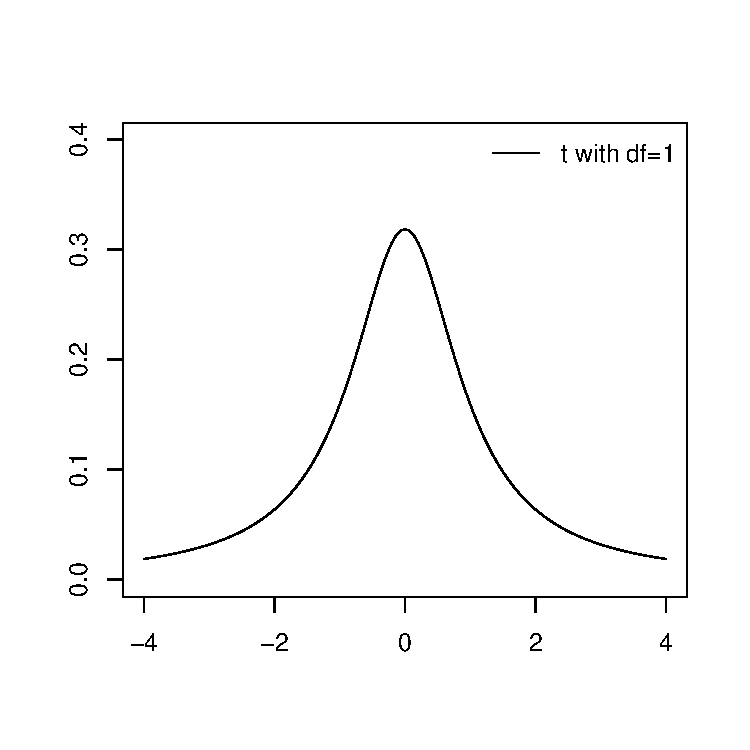
\includegraphics{figure/lec16-001}
\end{center}
\end{frame}
%-------------------------------------------------------------------------------


%-------------------------------------------------------------------------------
\addtocounter{framenumber}{-1}
\begin{frame}
\frametitle{$t$ Distribution Examples}
\setkeys{Gin}{width=0.85\textwidth}
\begin{center}
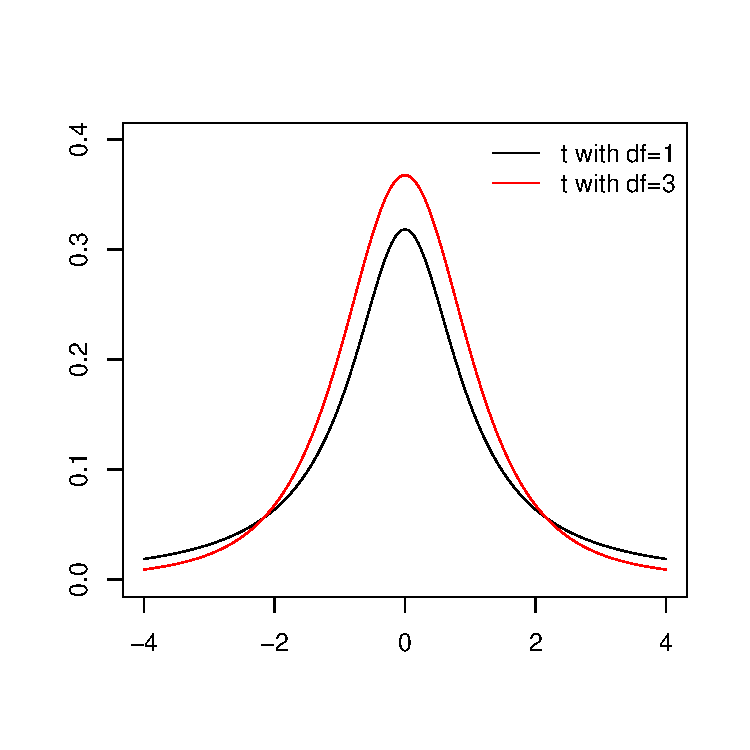
\includegraphics{figure/lec16-002}
\end{center}
\end{frame}
%-------------------------------------------------------------------------------


%-------------------------------------------------------------------------------
\addtocounter{framenumber}{-1}
\begin{frame}
\frametitle{$t$ Distribution Examples}
\setkeys{Gin}{width=0.85\textwidth}
\begin{center}
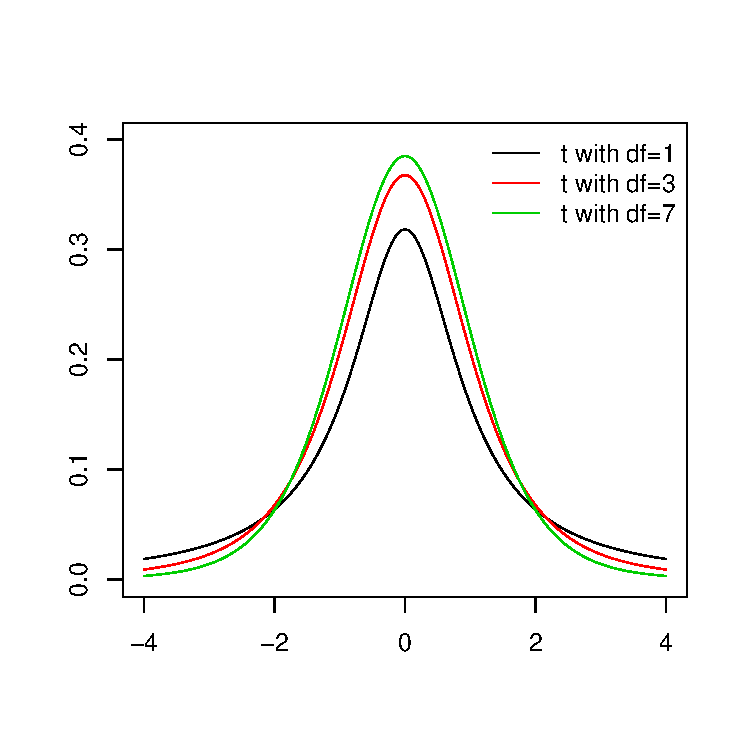
\includegraphics{figure/lec16-003}
\end{center}
\end{frame}
%-------------------------------------------------------------------------------


%-------------------------------------------------------------------------------
\addtocounter{framenumber}{-1}
\begin{frame}
\frametitle{$t$ Distribution Examples}
\setkeys{Gin}{width=0.85\textwidth}
\begin{center}
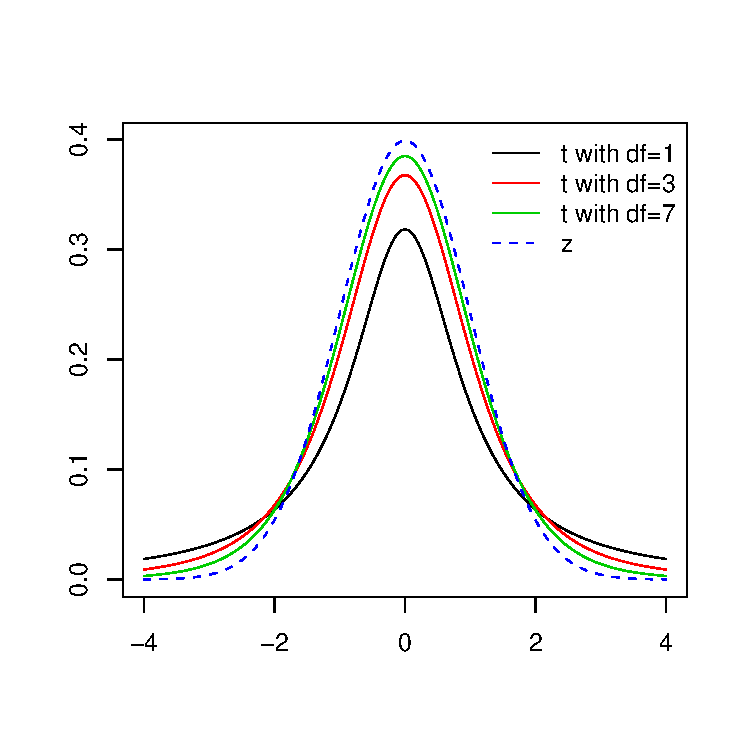
\includegraphics{figure/lec16-004}
\end{center}
\end{frame}
%-------------------------------------------------------------------------------


%-------------------------------------------------------------------------------
\begin{frame}
\frametitle{Conditions for Using t Distribution}
We use the $t$ distribution when you have a \blue{small sample} and

\begin{itemize}
\pause \item \blue{Independence}:
\begin{itemize}
\item $n \leq 10\% $ rule
\item or if we have an experiment or random process we check that each observation were independent
\end{itemize}
\pause \item \blue{Observations come from a nearly normal distribution}:  Difficult to verify with small data sets:
\begin{itemize}
\item Look at a histogram of the data
\item Consider whether any previous experiences alert us that the data may be normal
\end{itemize}
\end{itemize}  	
\end{frame}
%-------------------------------------------------------------------------------


%-------------------------------------------------------------------------------
\begin{frame}
\frametitle{$t$-Tables}
If $n=19$, we use $df=19-1=18$ and do a look up on the $t$-table on page 410:

\begin{center}
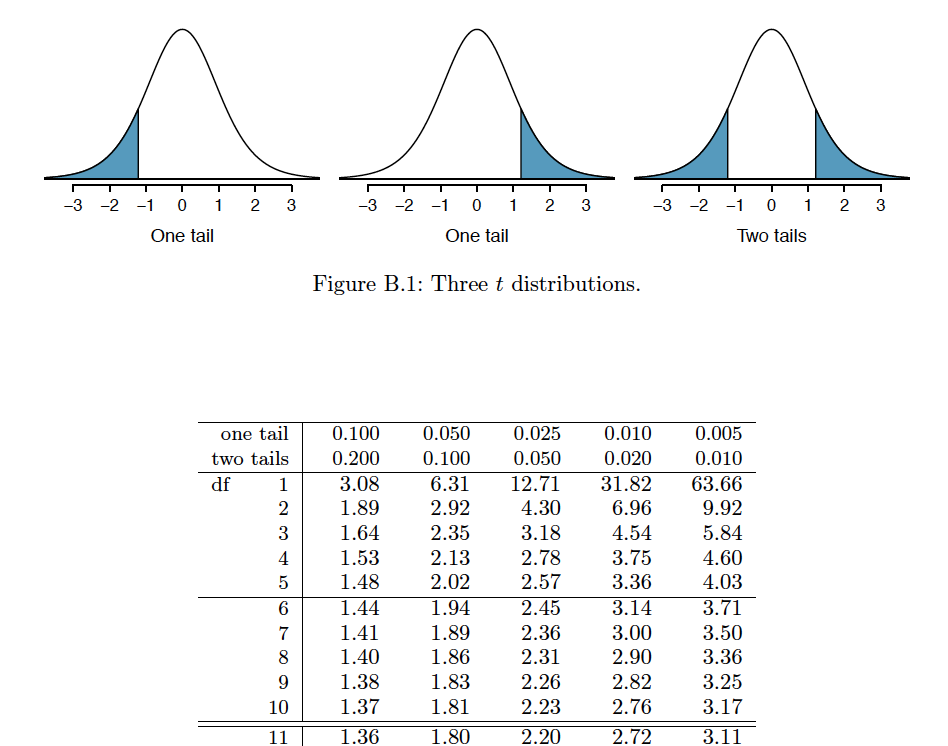
\includegraphics[width=0.75\textwidth]{figure/t.png}
\end{center}

\end{frame}
%-------------------------------------------------------------------------------


%-------------------------------------------------------------------------------
\begin{frame}
\frametitle{Confidence Intervals}

Confidence intervals:  Use $t^*_{df}$ instead of $z^*$
\[
\xbar \pm t_{df}^* SE = 
\left[
\overline{x} - t_{df}^* \times\frac{s}{\sqrt n}, \mbox{  }
\overline{x} + t_{df}^* \times\frac{s}{\sqrt n}
\right]
\]

So for example, to get a 95\% C.I. based on
\begin{eqnarray*}
n=18 \Rightarrow df=17 \Rightarrow t_{17}^*=2.11
\end{eqnarray*}

\end{frame}
%-------------------------------------------------------------------------------


%-------------------------------------------------------------------------------
\begin{frame}
\frametitle{$t$-Test Example}

Example 5.19 on page 252:  NYC is known as the city that never sleeps.  A random sample of 25 New Yorkers were asked how much sleep they get per night. Does the data below provide strong evidence that New Yorkers sleep less than 8 hours a night on average?  Set $\alpha=0.05$

\pause\vspace{0.5cm}
\begin{center}
\begin{tabular}{c|c|c|c|c}
$n$ & $\xbar$ & $s$ & min & max\\
\hline
25 & 7.73 & 0.77 & 6.17 & 9.78\\
\end{tabular}
\end{center}

\end{frame}
%-------------------------------------------------------------------------------


%-------------------------------------------------------------------------------
\begin{frame}
\frametitle{$t$-Test}
Conditions:
\begin{itemize}
\item \blue{Independence}: 25 is obviously less than 10\% of the population of NYC
\item \blue{Normality}: Not an exact science.  The halfway point of the min and max is 7.975, which is fairly close to $\xbar=7.73$.  So symmetric enough? 
\end{itemize}

\vspace{0.25cm}

The test statistic is the $t$-statistic:
\[
t = \frac{\overline{x}-\mbox{null value}}{SE} = \frac{\overline{x}-\mbox{null value}}{\frac{s}{\sqrt n}} = \frac{7.73 - 8}{\frac{0.77}{\sqrt{25}}} = -1.75
\]
Since $n=25$, $df=25-1=24$.
\end{frame}
%-------------------------------------------------------------------------------


%-------------------------------------------------------------------------------
\begin{frame}
\frametitle{$t$-Test}

$p$-Value. We use the $t$ distribution i.e. the $t$-table on page 410:
\begin{center}
\begin{tabular}{c|ccccc}
\hline
one-tail & 0.100 & 0.050 & 0.025 & 0.010 & 0.005\\
two-tail & 0.200 & 0.100 & 0.050 & 0.020 & 0.010\\
\hline
df = 24 & 1.32 & 1.71 & 2.06 & 2.49 & 2.80\\
\hline
\end{tabular}
\end{center}

Since 1.75 is in between one-tail values of 1.71 and 2.06 and by symmetry, the p-value is somewhere between 0.05 and 0.025. 

\vspace{0.5cm}

Decision: Since the p-value $< \alpha=0.05$, we reject $H_0$ that NY'ers sleep 8 hours a night at the $\alpha=0.05$ significance level in favor of the hypothesis they sleep more.
\end{frame}
%-------------------------------------------------------------------------------


%-------------------------------------------------------------------------------
\begin{frame}
\frametitle{History of $t$ Distribution}
The $t$ distribution was derived by William Sealy Gosset in 1908, a chemist/statistician at the Guinness Brewery in Dublin, Ireland.
\begin{center}
\includegraphics[width=2in]{figure/gosset.pdf}
\end{center}
\end{frame}
%-------------------------------------------------------------------------------


%-------------------------------------------------------------------------------
\begin{frame}
\frametitle{History of $t$ Distribution}
Gosset was concerned with \blue{small-sample statistics} about barley given that brewers are limited in the number of batches of beer they can brew.
\pause \vskip 0.5cm
Guinness prohibited its employees from publishing.  So Gosset had to use the pseudonym ``Student'' to conceal his identity.
\pause \vskip 0.5cm
In particular, the \blue{(Student's) t-test} is one of the most widely used statistical tests in the world.  
\end{frame}
%-------------------------------------------------------------------------------


%-------------------------------------------------------------------------------
\begin{frame}
\frametitle{History of $t$ Distribution}
In fact if you go to the Guinness Brewery at St James's Gate in Dublin, Ireland...
\begin{center}
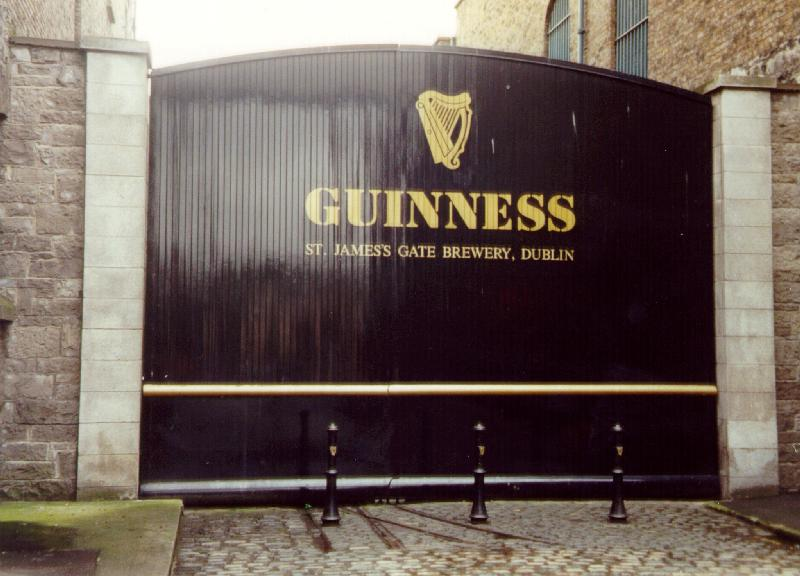
\includegraphics[width=3in]{figure/brewery.jpg}
\end{center}
\
\end{frame}
%-------------------------------------------------------------------------------


%-------------------------------------------------------------------------------
\begin{frame}
\frametitle{History of $t$ Distribution}
\begin{center}
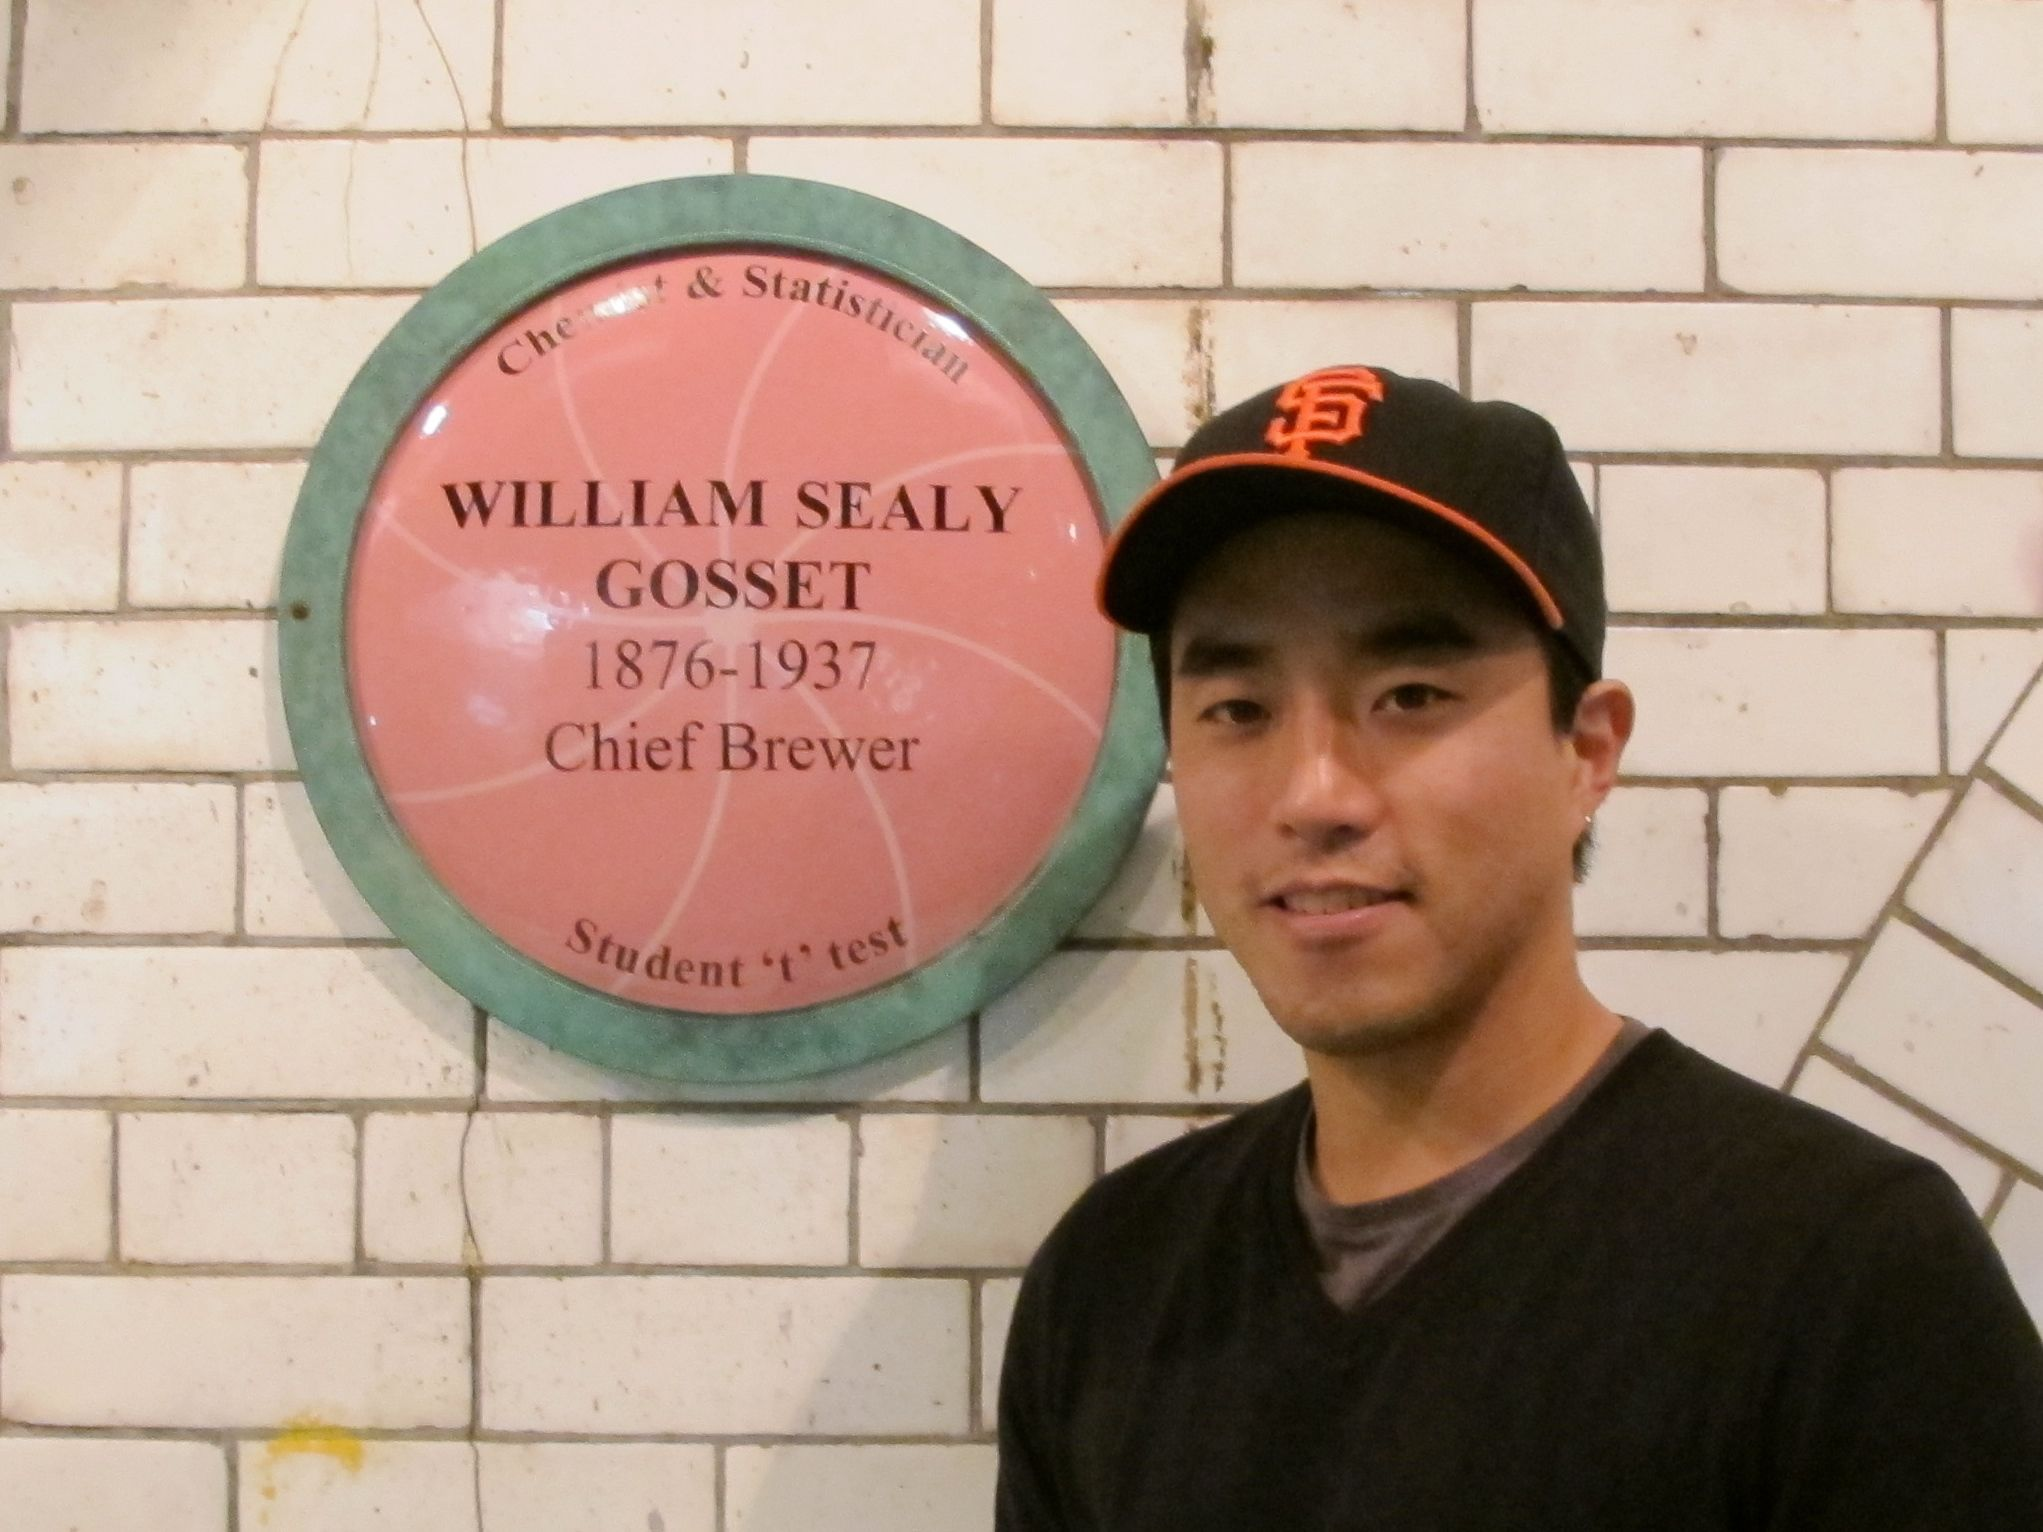
\includegraphics[width=0.9\textwidth]{figure/guinness.jpg}
\end{center}
\end{frame}
%-------------------------------------------------------------------------------


\end{document}













% Two-sample t-test


%------------------------------------------------------------------------------
\begin{frame}[fragile]
\frametitle{Question for Today}

In Lecture 7.2 (Chapter 5.2) we asked:  Did men ($n_m=45$) run faster than women ($n_w=55$) in the Cherry Blossom Race?
\begin{center}
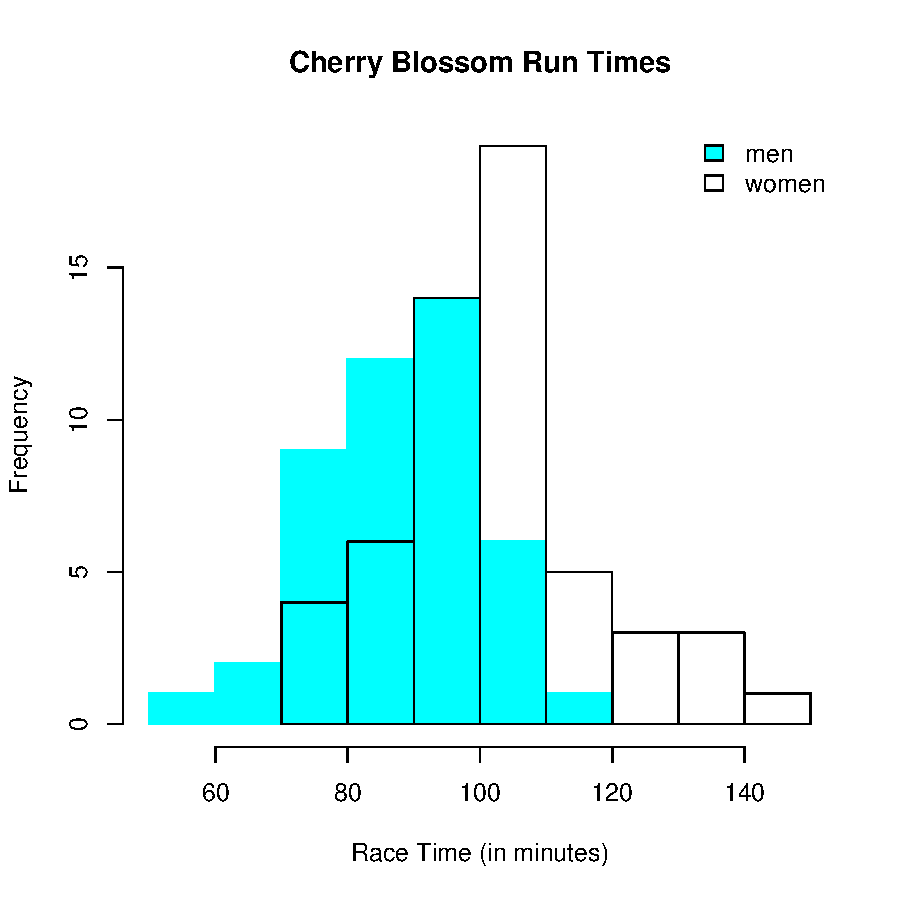
\includegraphics[width=0.4\textwidth]{figure/race.pdf}
\end{center}

\pause What can we say about $\mu_1 - \mu_2$ when $n_1$ and $n_2$ are both small?

\end{frame}
%------------------------------------------------------------------------------


%------------------------------------------------------------------------------
\begin{frame}[fragile]
\frametitle{Components}

Similarly to the last lecture on \blue{$t$-tests}, now we use the \blue{two sample $t$-test}: 

\begin{enumerate}
\pause \item The point estimate of $\mu_1 - \mu_2$ is $\xbar_1 - \xbar_2$
\pause \item The standard error of the sampling distribution
\[
SE_{\xbar_1 - \xbar_2} = \sqrt{\frac{s_1^2}{n_1} + \frac{s_2^2}{n_2}}
\]
\pause \item Confidence intervals using $t^*_{df}$
\pause \item Hypothesis tests using $t$-statistic
\end{enumerate}


\end{frame}
%------------------------------------------------------------------------------


%------------------------------------------------------------------------------
\begin{frame}[fragile]
\frametitle{Components}

But what degrees of freedom $df$ do we use?  

\vspace{0.25cm}

\pause The true formula for degrees of freedom is
\[
df = \frac{(s_1^2/n_1 + s_2^2/n_2)^2}{(s_1^2/n_1)^2/(n_1-1) + (s_2^2/n_2)^2/(n_2-1)}
\]

\pause Rather, for this class, use the smaller of $n_1$ and $n_2$ minus 1 i.e.
\[
\min(n_1, n_2) - 1
\]

\end{frame}
%------------------------------------------------------------------------------


%------------------------------------------------------------------------------
\begin{frame}[fragile]
\frametitle{Conditions of Two Sample $t$-Test}

\begin{itemize}
\item Both samples meet the conditions for using the $t$ distribution
\begin{itemize}
\pause \item Sample observations are nearly normal
\pause \item Sample observations are independent within their respective populations
\end{itemize}
\pause \item The two \blue{samples} are independent
\end{itemize}

\end{frame}
%------------------------------------------------------------------------------


%------------------------------------------------------------------------------
\begin{frame}[fragile]
\frametitle{Pooled Standard Deviation Estimate}
Say however, you suspect both populations have similar true population standard deviations $\sigma_1=\sigma_2=\sigma$.  

\pause \vspace{0.5cm}

If so, we can leverage this fact to make the $t$ distribution approach slightly more precise.


\end{frame}
%------------------------------------------------------------------------------


%------------------------------------------------------------------------------
\begin{frame}[fragile]
\frametitle{Pooled Standard Deviation Estimate}
The pooled standard deviation estimate is
\[
s^2_{pooled} = \frac{s_1^2\times(n_1 -1) + s_2^2 \times(n_2 -1)}{n_1 + n_2 - 2}
\]

\vspace{0.25cm}

\pause  So use $s^2_{pooled}$ instead of $s_1^2$ and $s_2^2$ in $SE$:
\[
SE_{\xbar_1 - \xbar_2} = \sqrt{\frac{s_1^2}{n_1} + \frac{s_2^2}{n_2}}
= \sqrt{\frac{s^2_{pooled}}{n_1} + \frac{s^2_{pooled}}{n_2}} =
\sqrt{s^2_{pooled}\left(\frac{1}{n_1} + \frac{1}{n_2}\right)}
\]

\end{frame}
%------------------------------------------------------------------------------


%------------------------------------------------------------------------------
\begin{frame}[fragile]
\frametitle{Pooled Standard Deviation Estimate}

You can think of $s^2_{pooled}$ as being very close to a \blue{weighted average} of the two sample standard deviations:

\begin{eqnarray*}
\pause s^2_{pooled} &=& s_1^2 \times\frac{n_1 - 1}{n_1 + n_2 - 2} + s_2^2 \times  \frac{n_2 - 1}{n_1+n_2-2}\\
\pause \mbox{close to} &\approx& s_1^2 \times\frac{n_1}{n_1 + n_2} + s_2^2 \times  \frac{n_2}{n_1+n_2}
\end{eqnarray*}

\vspace{0.5cm}

\pause The $-1$ and $-2$ are \blue{degrees of freedom} corrections.  

\end{frame}
%------------------------------------------------------------------------------


%------------------------------------------------------------------------------
\begin{frame}[fragile]
\frametitle{Pooled Standard Deviation Estimate}

So say $n_1=10$ and $n_2=20$, then 
\begin{eqnarray*}
s^2_{pooled} &\approx& s_1^2 \times\frac{10}{10 + 20} + s_2^2 \times  \frac{20}{10+20}\\
&\approx& s_1^2 \times\frac{1}{3} + s_2^2 \times  \frac{2}{3}\\
\end{eqnarray*}


\end{frame}
%------------------------------------------------------------------------------


%------------------------------------------------------------------------------
\begin{frame}[fragile]
\frametitle{Pooled Standard Deviation Estimate}
\blue{Benefits}:  If $\sigma$'s are equal, we have more precise model of the sampling distribution of $\xbar_1 - \xbar_2$

\vspace{0.5cm}

\pause \blue{Caveats}:  Only pool when background research/intuition indicates the population $\sigma_1$ and $\sigma_2$ of the two groups are nearly equal.  
\end{frame}
%------------------------------------------------------------------------------
